\documentclass[12pt]{article}

\usepackage{sbc-template}

\usepackage{graphicx,url}

%\usepackage[brazil]{babel}
%\usepackage[portuguese]{babel}
\usepackage[latin1]{inputenc}

\usepackage[T1]{fontenc}
\usepackage{pgfplots}

\sloppy

\title{Instructions for Authors of SBC Conferences\\ Papers and Abstracts}

\author{Marino Souza dos Santos\inst{1} }


\address{Departamento de Ci�ncia da Computa��o -- Instituto de Matem�tica\\Universidade Federal Bahia
  (UFBA)\\
  40.170-110 -- Salvador -- BA -- Brazil
  \email{marino@dcc.ufba.br}
}

\begin{document}

\maketitle

\begin{abstract}
  Lorem ipsum dolor sit amet, consectetur adipisicing elit, sed do eiusmod
  tempor incididunt ut labore et dolore magna aliqua. Ut enim ad minim veniam,
  quis nostrud exercitation ullamco laboris nisi ut aliquip ex ea commodo
  consequat. Duis aute irure dolor in reprehenderit in voluptate velit esse
  cillum dolore eu fugiat nulla pariatur. Excepteur sint occaecat cupidatat non
  proident, sunt in culpa qui officia deserunt mollit anim id est laborum.
\end{abstract}

\begin{resumo}
  Lorem ipsum dolor sit amet, consectetur adipisicing elit, sed do eiusmod
  tempor incididunt ut labore et dolore magna aliqua. Ut enim ad minim veniam,
  quis nostrud exercitation ullamco laboris nisi ut aliquip ex ea commodo
  consequat. Duis aute irure dolor in reprehenderit in voluptate velit esse
  cillum dolore eu fugiat nulla pariatur. Excepteur sint occaecat cupidatat non
  proident, sunt in culpa qui officia deserunt mollit anim id est laborum.
\end{resumo}


\section{General Information}

Lorem ipsum dolor sit amet, consectetur adipisicing elit, sed do eiusmod
tempor incididunt ut labore et dolore magna aliqua. Ut enim ad minim veniam,
quis nostrud exercitation ullamco laboris nisi ut aliquip ex ea commodo
consequat. Duis aute irure dolor in reprehenderit in voluptate velit esse
cillum dolore eu fugiat nulla pariatur. Excepteur sint occaecat cupidatat non
proident, sunt in culpa qui officia deserunt mollit anim id est laborum.

\section{First Page} \label{sec:firstpage}

Lorem ipsum dolor sit amet, consectetur adipisicing elit, sed do eiusmod
tempor incididunt ut labore et dolore magna aliqua. Ut enim ad minim veniam,
quis nostrud exercitation ullamco laboris nisi ut aliquip ex ea commodo
consequat. Duis aute irure dolor in reprehenderit in voluptate velit esse
cillum dolore eu fugiat nulla pariatur. Excepteur sint occaecat cupidatat non
proident, sunt in culpa qui officia deserunt mollit anim id est laborum \cite{creator}.

Lorem ipsum dolor sit amet, consectetur adipisicing elit, sed do eiusmod
tempor incididunt ut labore et dolore magna aliqua. Ut enim ad minim veniam,
quis nostrud exercitation ullamco laboris nisi ut aliquip ex ea commodo
consequat. Duis aute irure dolor in reprehenderit in voluptate velit esse
cillum dolore eu fugiat nulla pariatur. Excepteur sint occaecat cupidatat non
proident, sunt in culpa qui officia deserunt mollit anim id est laborum \cite{donator}.

\section{Proceedings}

Lorem ipsum dolor sit amet, consectetur adipisicing elit, sed do eiusmod
tempor incididunt ut labore et dolore magna aliqua. Ut enim ad minim veniam,
quis nostrud exercitation ullamco laboris nisi ut aliquip ex ea commodo
consequat. Duis aute irure dolor in reprehenderit in voluptate velit esse
cillum dolore eu fugiat nulla pariatur. Excepteur sint occaecat cupidatat non
proident, sunt in culpa qui officia deserunt mollit anim id est laborum.

\begin{figure}
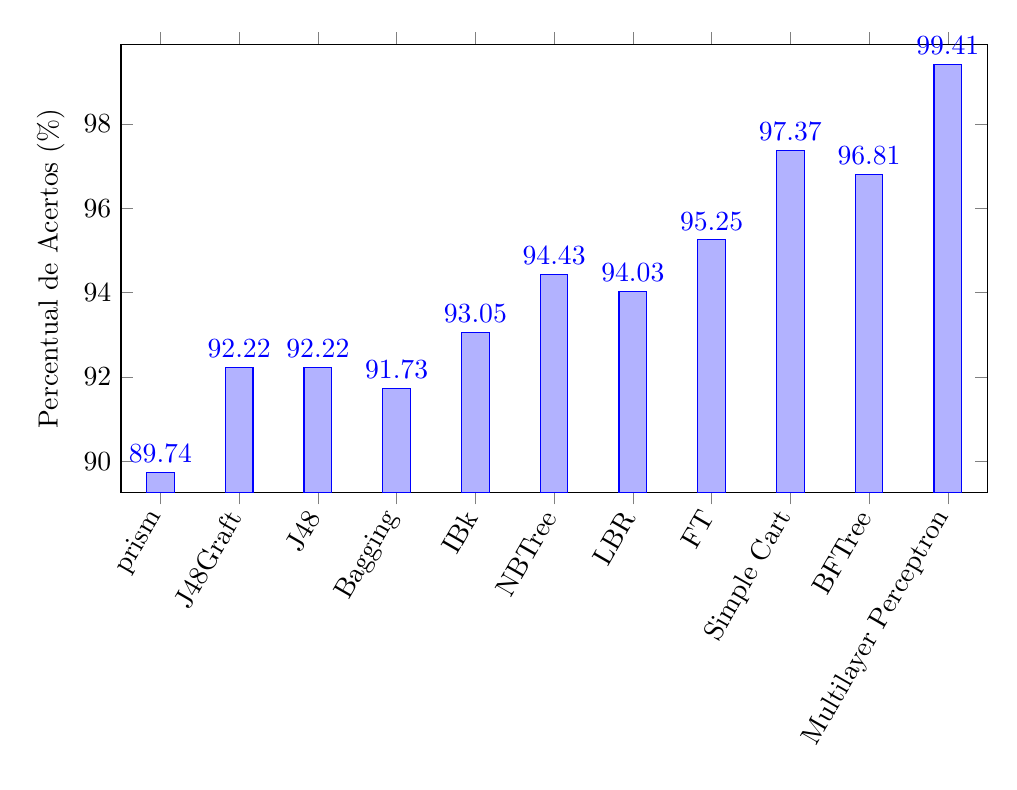
\begin{tikzpicture} \begin{axis}[
    ybar, x=1cm,
    enlargelimits=0.05,
    legend style={at={(0.5,-0.2)},
    anchor=north,legend columns=-1},
    ylabel={Percentual de Acertos (\%)},
    symbolic x coords={prism,J48Graft,J48,%
     Bagging,IBk, NBTree, LBR, FT, Simple Cart, BFTree, Multilayer Perceptron},
     xtick=data,
     nodes near coords, nodes near coords align={vertical},
    x tick label style={rotate=60,anchor=east}, ]
\addplot coordinates {(prism,89.74) (J48Graft,92.22) (J48,92.22) (Bagging,91.73) (IBk,93.05) (NBTree,94.43) (LBR, 94.03)
    (FT, 95.25) (Simple Cart, 97.37) (BFTree, 96.81) (Multilayer Perceptron, 99.41) };
\end{axis}
\end{tikzpicture}
\caption{Ranking do percentual de acerto dos algoritmos}
\label{figure:ranking}
\end{figure}


\section{Sections and Paragraphs}

Lorem ipsum dolor sit amet, consectetur adipisicing elit, sed do eiusmod
tempor incididunt ut labore et dolore magna aliqua. Ut enim ad minim veniam,
quis nostrud exercitation ullamco laboris nisi ut aliquip ex ea commodo
consequat. Duis aute irure dolor in reprehenderit in voluptate velit esse
cillum dolore eu fugiat nulla pariatur. Excepteur sint occaecat cupidatat non
proident, sunt in culpa qui officia deserunt mollit anim id est laborum.

\subsection{Subsections}

Lorem ipsum dolor sit amet, consectetur adipisicing elit, sed do eiusmod
tempor incididunt ut labore et dolore magna aliqua. Ut enim ad minim veniam,
quis nostrud exercitation ullamco laboris nisi ut aliquip ex ea commodo
consequat. Duis aute irure dolor in reprehenderit in voluptate velit esse
cillum dolore eu fugiat nulla pariatur. Excepteur sint occaecat cupidatat non
proident, sunt in culpa qui officia deserunt mollit anim id est laborum.

\begin{table}[h]
  \begin{center}
    \begin{tabular}{ l | l | l | l}
      \hline
      Dom�nio & Inst�ncias & Atributos & Tipo de Classe \\ \hline
      Bresat Cancer Winscosin & 699 & 9 & Discreta \\ \hline
    \end{tabular}
    \caption[Dados do dom�nio]{Dados do conjunto de dados Breast Cancer Winscosin\cite{donator:92}}
    \label{table:dataset}
  \end{center}
\end{table}

O dom�nio do \textit{Breast Cancer Winscosin dataset} disponibilizado por \cite{donator:92} possuia 10 atributos mais a classe. Para este experimento o primeiro atributo (\texttt{ID de Pacientes}) foi omitido por n�o ser significante para a an�lise ficando com a seguinte configura��o.

\begin{table}
  \begin{center}
    \begin{tabular}{ l | l }
      \hline
      \multicolumn{2}{c}{ \bfseries Base do Hospital de Winscosin} \\ \hline
      \bfseries Atributo & \bfseries Intervalo inteiro\\ \hline
      Clump Thickness & Entre 1 e 10 \\
      Uniformity of Cell Size & Entre 1 e 10 \\
      Uniformity of Cell Shape & Entre 1 e 10 \\
      Marginal Adhesion & Entre 1 e 10 \\
      Single Epithelial Cell Size & Entre 1 e 10 \\
      Bare Nuclei & Entre 1 e 10 \\
      Bland Chromatin & Entre 1 e 10 \\
      Normal Nucleoli & Entre 1 e 10 \\
      Mitoses & Entre 1 e 10 \\
      \hline
    \end{tabular}
  \end{center}
  \caption{ As classes s�o escritas como 2 para ben�ngo e 4 para mal�gno}
  \label{table:disposicao-atributos}
\end{table}

\section{Figures and Captions}\label{sec:figs}


Lorem ipsum dolor sit amet, consectetur adipisicing elit, sed do eiusmod
tempor incididunt ut labore et dolore magna aliqua. Ut enim ad minim veniam,
quis nostrud exercitation ullamco laboris nisi ut aliquip ex ea commodo
consequat. Duis aute irure dolor in reprehenderit in voluptate velit esse
cillum dolore eu fugiat nulla pariatur. Excepteur sint occaecat cupidatat non
proident, sunt in culpa qui officia deserunt mollit anim id est laborum.

\section{References}

Bibliographic references must be unambiguous and uniform.  We recommend giving
the author names references in brackets, e.g. \cite{weka:09}.

\bibliographystyle{sbc}
\bibliography{sbc-template}

\end{document}
